\chapter{Methodology}
We developed a drone based monitoring and visualization service for the farmers to analyse their fields using an easy to use interface of an android application. The application serves as an intermediary between the local Drone dispatch station. The dispatch stations are already present in Uttrakhand as UKSWAN (Uttrakhand State Wide Area Network).\\ 
Drone based scanning of a large area for both visible and near-infrared light by stitching images on basis of their location could help track changes in plants at large scale and identify the distribution pattern very precisely.\\
The whole process can be broken down to several steps, starting with polygon formation of the area to be processed or the crop cover. Trajectory of the drone is planned by an open source library , Mission Planner, with a ground station interface compatible with ArduPilot. This is tended to be the basic wire-line platform for the drone. Flight trajectories are planned by polygon points in the AUTO mode of the drone flight. The drone is a 250mm chassis drone equipped with APM 2.8, an  ArduPilot based flight controller, which can be given GPS coordinates of the points to be traversed through a remote server (can be a phone) or through direct instructions to the flight controller before beginning the flight using the firmware ArduPilot 5.3.3. We use NoIR camera with a red-light filter, allowing for only near Infra-Red wavelengths to be captured in the red channel of the image. We use a Raspberry Pi to trigger the camera to capture the images of the field in their field of vision at particular distances covered by the drone. Hence, as the drone traverses the trajectory planned by Motion Planning library to cover the crop field, images are taken by the drone in RGB, with the red channel having near IR. 
The taken images are then collected according to the optimum levels of frontal and side overlaps (60\% and 35\% respectively) for stitching the images into one image.\\
\begin{figure}[H]
    \centering
    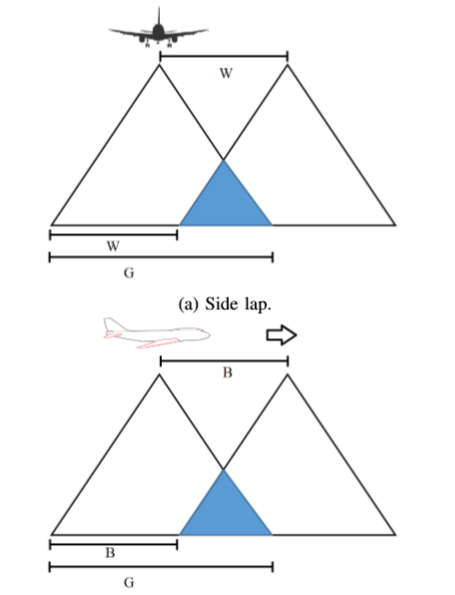
\includegraphics[width=0.7\linewidth]{SummerInterReport/project/Images-Major/overlap.png}
    \caption{Overlap and Stitching Source: \cite{one}}
    \label{fig:compEy}
\end{figure}

From the camera, a single crop field image of the whole field is made by processing the capture images at given time-stamps according to their metadata correlating with the time-stamps in the GPS tag coordinates found in the MAP log in ardupilot. A stitched photograph is formed which is then corrected to give an orthomosaic using OpenDroneMap(ODM) library which is open source. An orthomosaic is taken for measuring true distances, because it is an accurate representation of the Earth's surface, having been adjusted for topographic relief, lens distortion, and camera tilt, which replaces the uncorrected stitched photo.\\
We can process the image to find out the Normalized Difference Vegetation Index (NDVI) which is a clear indicator of crop chlorophyll levels, directly implying the crop health. The NDVI is the normalized difference of the reflectances of near IR and Red(or Blue) intensities as 
\begin{equation}
    (\rho nir - \rho red) / (\rho nir + \rho red)
\end{equation} A low NDVI indicates loss of either water or the nutrients in the crop field. We use the blue(i.e. red light) filter to get an IR Thermal imagery which defines the water stress level at different spatial regions due to the moisture held in different parts of the crop field (hotter due to thermal holding capacity of the water).
\\
This precision agricultural data is presented to a farmer via a simple application which can be used by them to call for the drone support and the whole report of their field is presented as an easy to understand info-graphic. Such approach could also open the scope of predictive analysis to execute automated alert to the farmers, potentially improving the crop productivity by more than 20\%.


\section{Drone}
The drone is programmed using the Mission Planner. 
\begin{figure}[H]
    \centering
    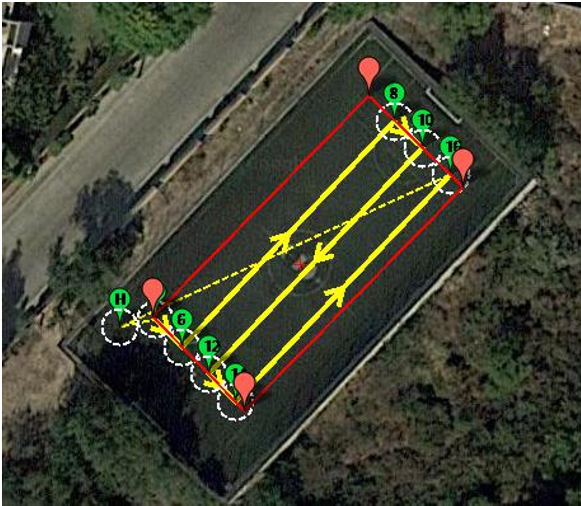
\includegraphics[width=0.7\linewidth]{SummerInterReport/project/Images-Major/flightTraj.png}
    \caption{Flight Trajectory generated by the Mission Planner flight plan tool; Source: \cite{one}}
    \label{fig:compEy}
\end{figure}
 In order to obtain aerial imagery, the first step is to establish a trajectory that the UAV will follow according to the area of interest. For deciding the trajectory, we have used Mission Planner. Mission Planner is a ground station interface compatible with the ArduPilot platform that can be connected to any flight controller based on APM2.8 autopilot. Trajectories can be performed using manual flight modes like STABILIZE, LOITER, and ALT-HOLD. They can also be planned manually using way points at specific locations. These points will guide the UAV. Another way to specify flights trajectories is using polygon points which will automatically generate a flight trajectory covering a desired area. These kind of trajectories are performed in AUTO mode. The flight trajectory used in this procedure will be planned according to the use of polygon points around the area of interest. 
\begin{figure}[H]
    \centering
    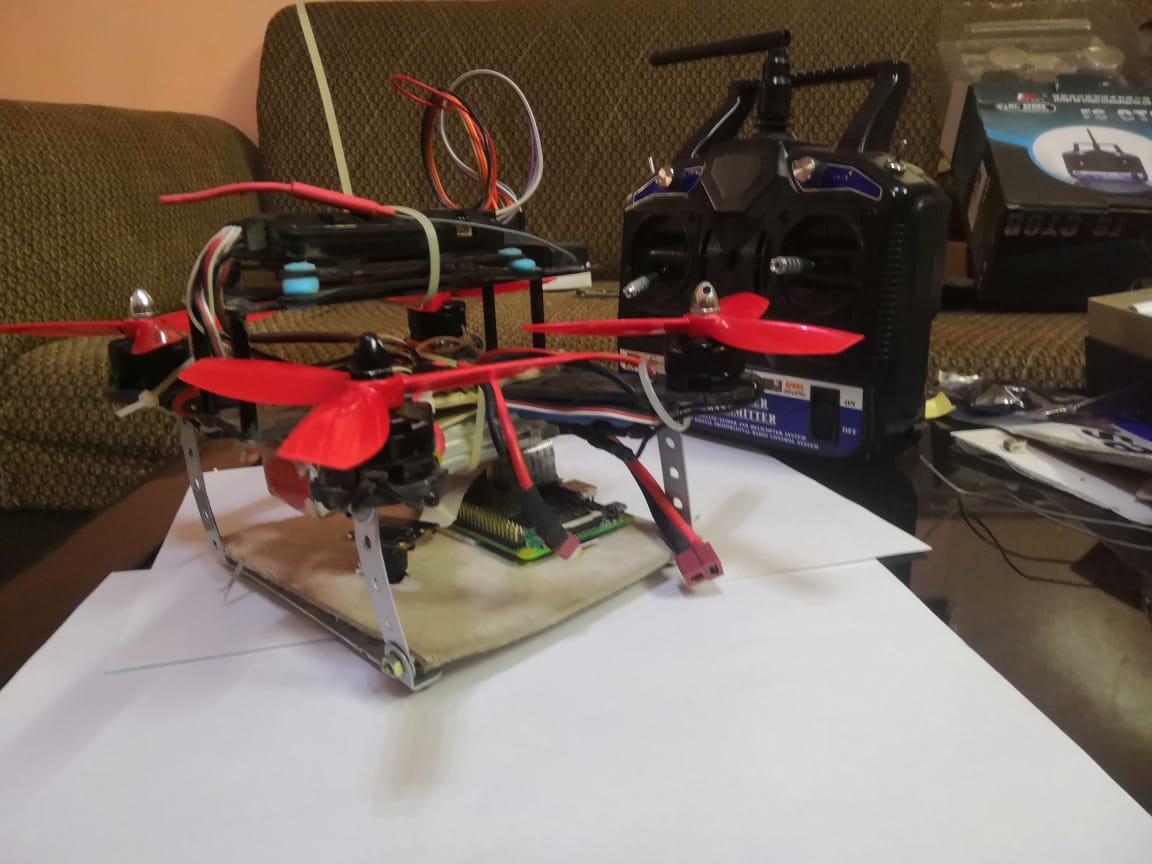
\includegraphics[width=0.7\linewidth]{SummerInterReport/project/Images-Major/complete_drone.jpeg}
    \caption{Complete Drone System generated}
    \label{fig:compEy}
\end{figure}

\section{Data Acquisition and Processing}
The formula to calculate NDVI requires us to know the amount of Near Infrared(NIR) light reflected by the plants and the Red light reflected by the plants. The problem arises when we have to establish such a system on a drone. Hence, it needs to be simple, light and efficient. We worked on three different methods to find out an approximate NDVI keeping in consideration accuracy as well as the cost factor of the overall system.
\subsection{Method 1}
In this method, we acquire the NIR from the Red channel of the Raspberry Pi NoIR camera as it has its infrared filter removed. We use a normal Pi Camera for the identifying the Red light reflected back. But attaching two camera to a Raspberry Pi is not possible without an adapter which costs about Rs. 7000. Rather, attaching two Raspberry Pis is a better and cheaper alternative. Hence each camera has a controlling Raspberry Pi, both triggered to click photos at the same time by the APM2.8
\\
On being triggered, the python script takes a snapshot using the OpenCV package and puts it up on the LAN shared by the two Raspberry Pis using http.server package of Python. Matrix manipulation is done by dividing the difference of the red channel values of both the photos from their sum to calculate NDVI.
\\
NDVI is a ratio from -1 to 1. It is then scaled to range of pixel values(0-255) using the formula (NDVI+1)*255/2. It is then converted to uint8 format from float. After this, the resultant matrix has gradient applied to it using OpenCV and is then further displayed on the web socket

\begin{figure}[H]
    \centering
    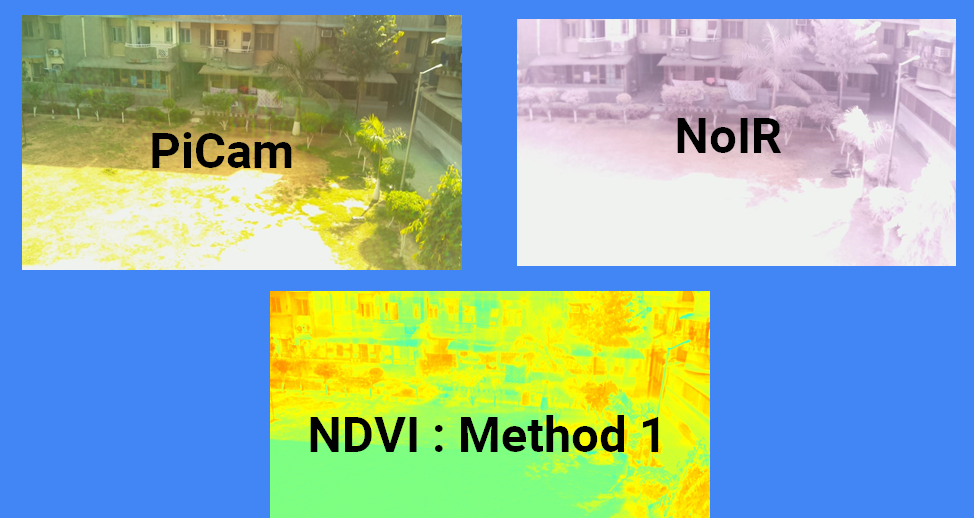
\includegraphics[width=\linewidth]{SummerInterReport/project/Images-Major/ndvi_one.png}
    \caption{Method 1 NDVI calculation}
    \label{fig:compEy}
\end{figure}

\subsubsection{Limitations}
\begin{enumerate}
    \item Connecting two Raspberry Pi leads to synchronization problems in the photos taken due to possible randomly unequal lag supplemented with the dynamics of it being on a drone.
    \item The photos have to be overlapping for the NDVI calculated to be accurate. To achieve this, we need to process the images snapped in accordance to the position of the cameras relative to each other, which may vary from installation to installation, making it a cumbersome task to achieve with high accuracy.
    \item Most importantly, while the formula requires value of NIR reflected, the red channel of the NoIR camera records Red+NIR, leading to a very dampened ratio.
\end{enumerate}
\subsection{Method 2}
In this method, rather than working on individual channels, we work on the intensity of the photos recorded by the two camera. It has the same setup as method 1, but the processing is different. The difference here is that the images are converted to gray-scale for processing.
\\
The conversion of images to gray-scale using OpenCV leads to the images having only one channel. The NIR intensity is replaced by the intensity of the NoIR camera's captured gray-scale image while the Red instensity is replaced by the normal Pi camera's captured gray-scale image to calculate NDVI.
\\
The calculated ratio is then, same as method 1, is mapped to obtain an infographic depicting an approximate value of NDVI

\begin{figure}[H]
    \centering
    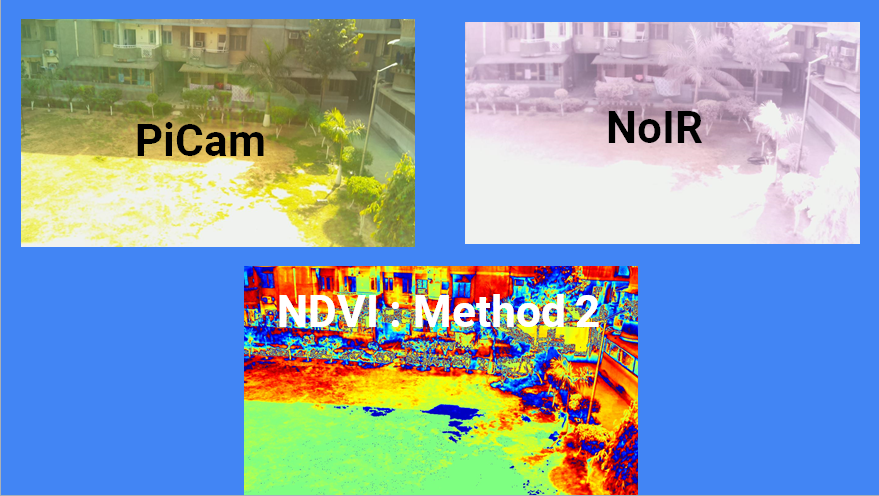
\includegraphics[width=\linewidth]{SummerInterReport/project/Images-Major/ndvi_two.png}
    \caption{Method 2 NDVI calculation}
    \label{fig:compEy}
\end{figure}

\subsubsection{Limitations}
\begin{enumerate}
    \item Same as Method 1
    \item Same as Method 1
    \item It is dependent on light intensity of the images, it is very sensitive to shadows and light intensity changes leading to disparity in calculated NDVI. 
\end{enumerate}
\subsection{Method 3}
NDVI works with Infrared and Red because while Infrared is mostly reflected back by healthy plants, the red light is mostly absorbed by them. But it is not only red light that is absorbed. The leaves(having chlorophyll) also absorb the Blue light, leading to the leaves appearing green to us. Hence, blue light reflected can also be used to calculate NDVI instead of red light.
\\
A blue film filter has the capability to prevent any red light from passing. This in conjunction with the Pi NoIR camera helps us receive intensity of pure NIR(theoretically) in the Red channel of the captured image while we get intensity of Blue light reflected from the blue channel of the image. This type of image is called Infrablue.

\begin{figure}[H]
    \centering
    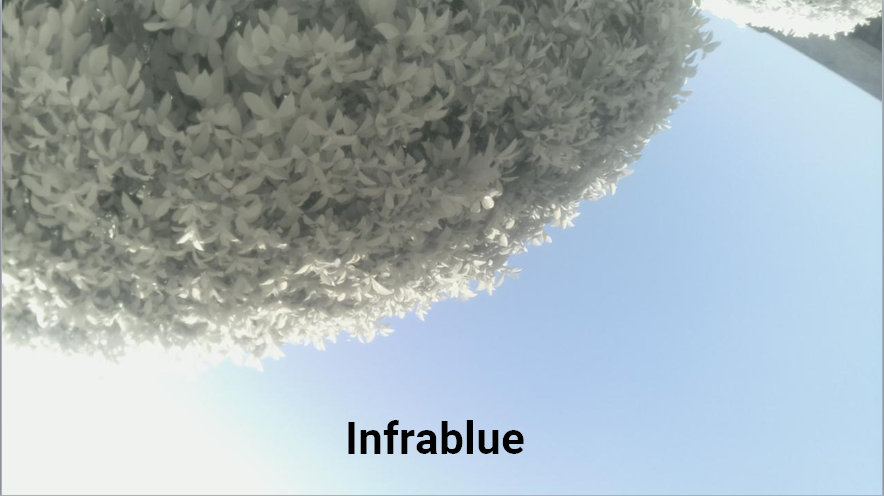
\includegraphics[width=0.7\linewidth]{SummerInterReport/project/Images-Major/infrablue.png}
    \caption{Infrablue Obtained in Method 3 of NDVI calculation}
    \label{fig:compEy}
\end{figure}
\begin{figure}[H]
    \centering
    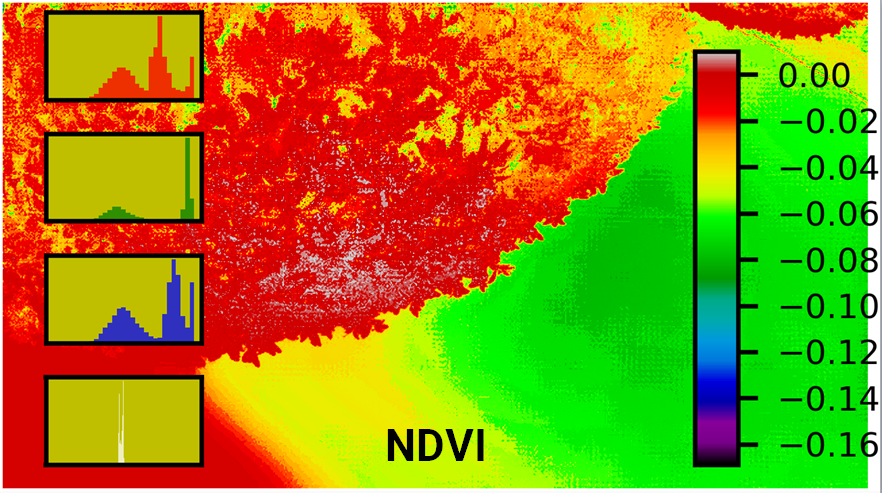
\includegraphics[width=\linewidth]{SummerInterReport/project/Images-Major/ndvi_three.png}
    \caption{Method 3 of NDVI calculation}
    \label{fig:compEy}
\end{figure}

In this method, we require only one Raspberry Pi connected to a Pi NoIR camera with an additional red light filter. The image is captured when triggered by the APM2.8 using OpenCV. Then the NDVI ratio is calculated by using the intensity of blue instead of red and taking intensity of NIR from the red channel of the image. The ratio is then extrapolated to pixel values and a gradient is applied for a pictorial representation in accordance to the minimum and maximum value of the ratio calculated. Further, histograms can be plotted using Matplotlib package for analysing the data.
\\
Method 3 solved all the limitations of the previous methods and proved to be the most optimum method to determine crop health using NDVI.
